\documentclass[10pt,a4paper]{article}
\usepackage[utf8]{inputenc}
\usepackage[german]{babel}
\usepackage{mathrsfs}
\usepackage{amsmath}
\usepackage{amsfonts}
\usepackage{amssymb}
\usepackage{amsthm}
\usepackage{graphicx}
\usepackage{float}
\usepackage[left=2cm,right=2cm,top=2cm,bottom=2cm]{geometry}

\begin{document}

\section{Aufgabe 1}
Die Laufzeit ist $\Theta(n \cdot N)$.

\section{Aufgabe 2}
Ich werde in allen Teilen Min-Heaps betrachten.

\subsection{Suchen des Maximums}
In einem Min-Heap muss das Maximum in den Blättern sein.
Man kann aber keine weitere Aussage über die Position des Maximums treffen, sodass man in unserer üblichen Arraydarstellung die letzten $n / 2$ Knoten in linearer Zeit $\mathcal{O}(n)$ nach dem Maximum durchsuchen muss.

\subsection{Entfernen des Maximums}
Wenn man das Maximum nun gefunden hat, entfernt man es und ersetzt es mit dem letzten Element im Feld (der rechteteste Knoten in der untersten Ebene).
Dieses könnte jetzt allerdings die Heap-Eigenschaften verletzen, sodass man es solange nach oben schiebt, bis die Heap-Eigenschaft wiederhergestellt ist.
Da der Heap $\log n$ Stufen hat, benötigt dies nur sublineare Zeit und die gesamte Operation läuft wieder in $\mathcal{O}(n)$.

\subsection{Suchen des Minimums}
Da das Minimum eines Min-Heaps per Definition immer in der Wurzel steht, lässt es sich einfach durch Inspektion von $A[0]$ in $\mathcal{O}(1)$ bestimmen.

\subsection{Entfernen des Minimums}
Das Minimum zu entfernen, kann durch Entfernen der Wurzel und anschließendes Reparieren des Heaps durch Versickern des letztens Elements in $\mathcal{O}(\log n)$ durchgeführt werden.

\subsection{Suchen eines beliebigen Elements}
Ich nehme mal an, dass das bedeuten soll, zu prüfen, ob ein gegebenes Element im Heap vorhanden ist.
Da man nicht allgemein vorhersagen kann, in welchem Zweig eines Heaps ein Element landen wird, kommt man hier nicht drum herum, alle Elemente in $\mathcal{O}(n)$ zu überprüfen.

\subsection{Entfernen eines beliebigen Elements}
Zuerst bestimmt man die Position des Elements.
Wenn es sich im Heap befindet, entfernt man es und ersetzt es mit dem letzten Element.
Dieses könnte jedoch die Heap-Eigenschaft verletzen, was man mit dem Algorithmus der Heap-Erstellung beseitigt.
Die beiden Kind-Heaps des eingesetzten Elements, sind noch gültige Heaps, sodass man von dort aus bis zur Wurzel in $\mathcal{O}(n)$ repariert, was dann auch die Gesamtlaufzeit der Operation wäre.

\section{Aufgabe 3}
\begin{proof}
  Sei $j = 0$.
  \begin{equation}
    \sum_{k = 1}^{-1} 2^{k - 1} (-k) = 0 = 2^{0} - 1
  \end{equation}
  
  Sei $j > 0 \in \mathbb{N}$ und die Aussage sei wahr für $j - 1$.
  \begin{align*}
    \sum_{k = 1}^{j - 1} 2^{k - 1} (j - k) & = 2^{j - 2} (j - j + 1) + \sum_{k = 1}^{j - 2} 2^{k - 1} (j - 1 - k) + \sum_{k = 1}^{j - 2} 2^{k - 1}\\
    & = 2^{j - 2} + 2^{j - 1} - j + \sum_{k = 1}^{j - 2} 2^{k - 1}\\
    & = 2^{j - 2} + 2^{j - 1} - j + 2^{j - 2} - 1\\
    & = 2^{j - 1} + 2^{j - 1} - j - 1\\
    & = 2^{j} - (j + 1)
  \end{align*}
\end{proof}

\section{Aufgabe 4}

\begin{figure}[H]
  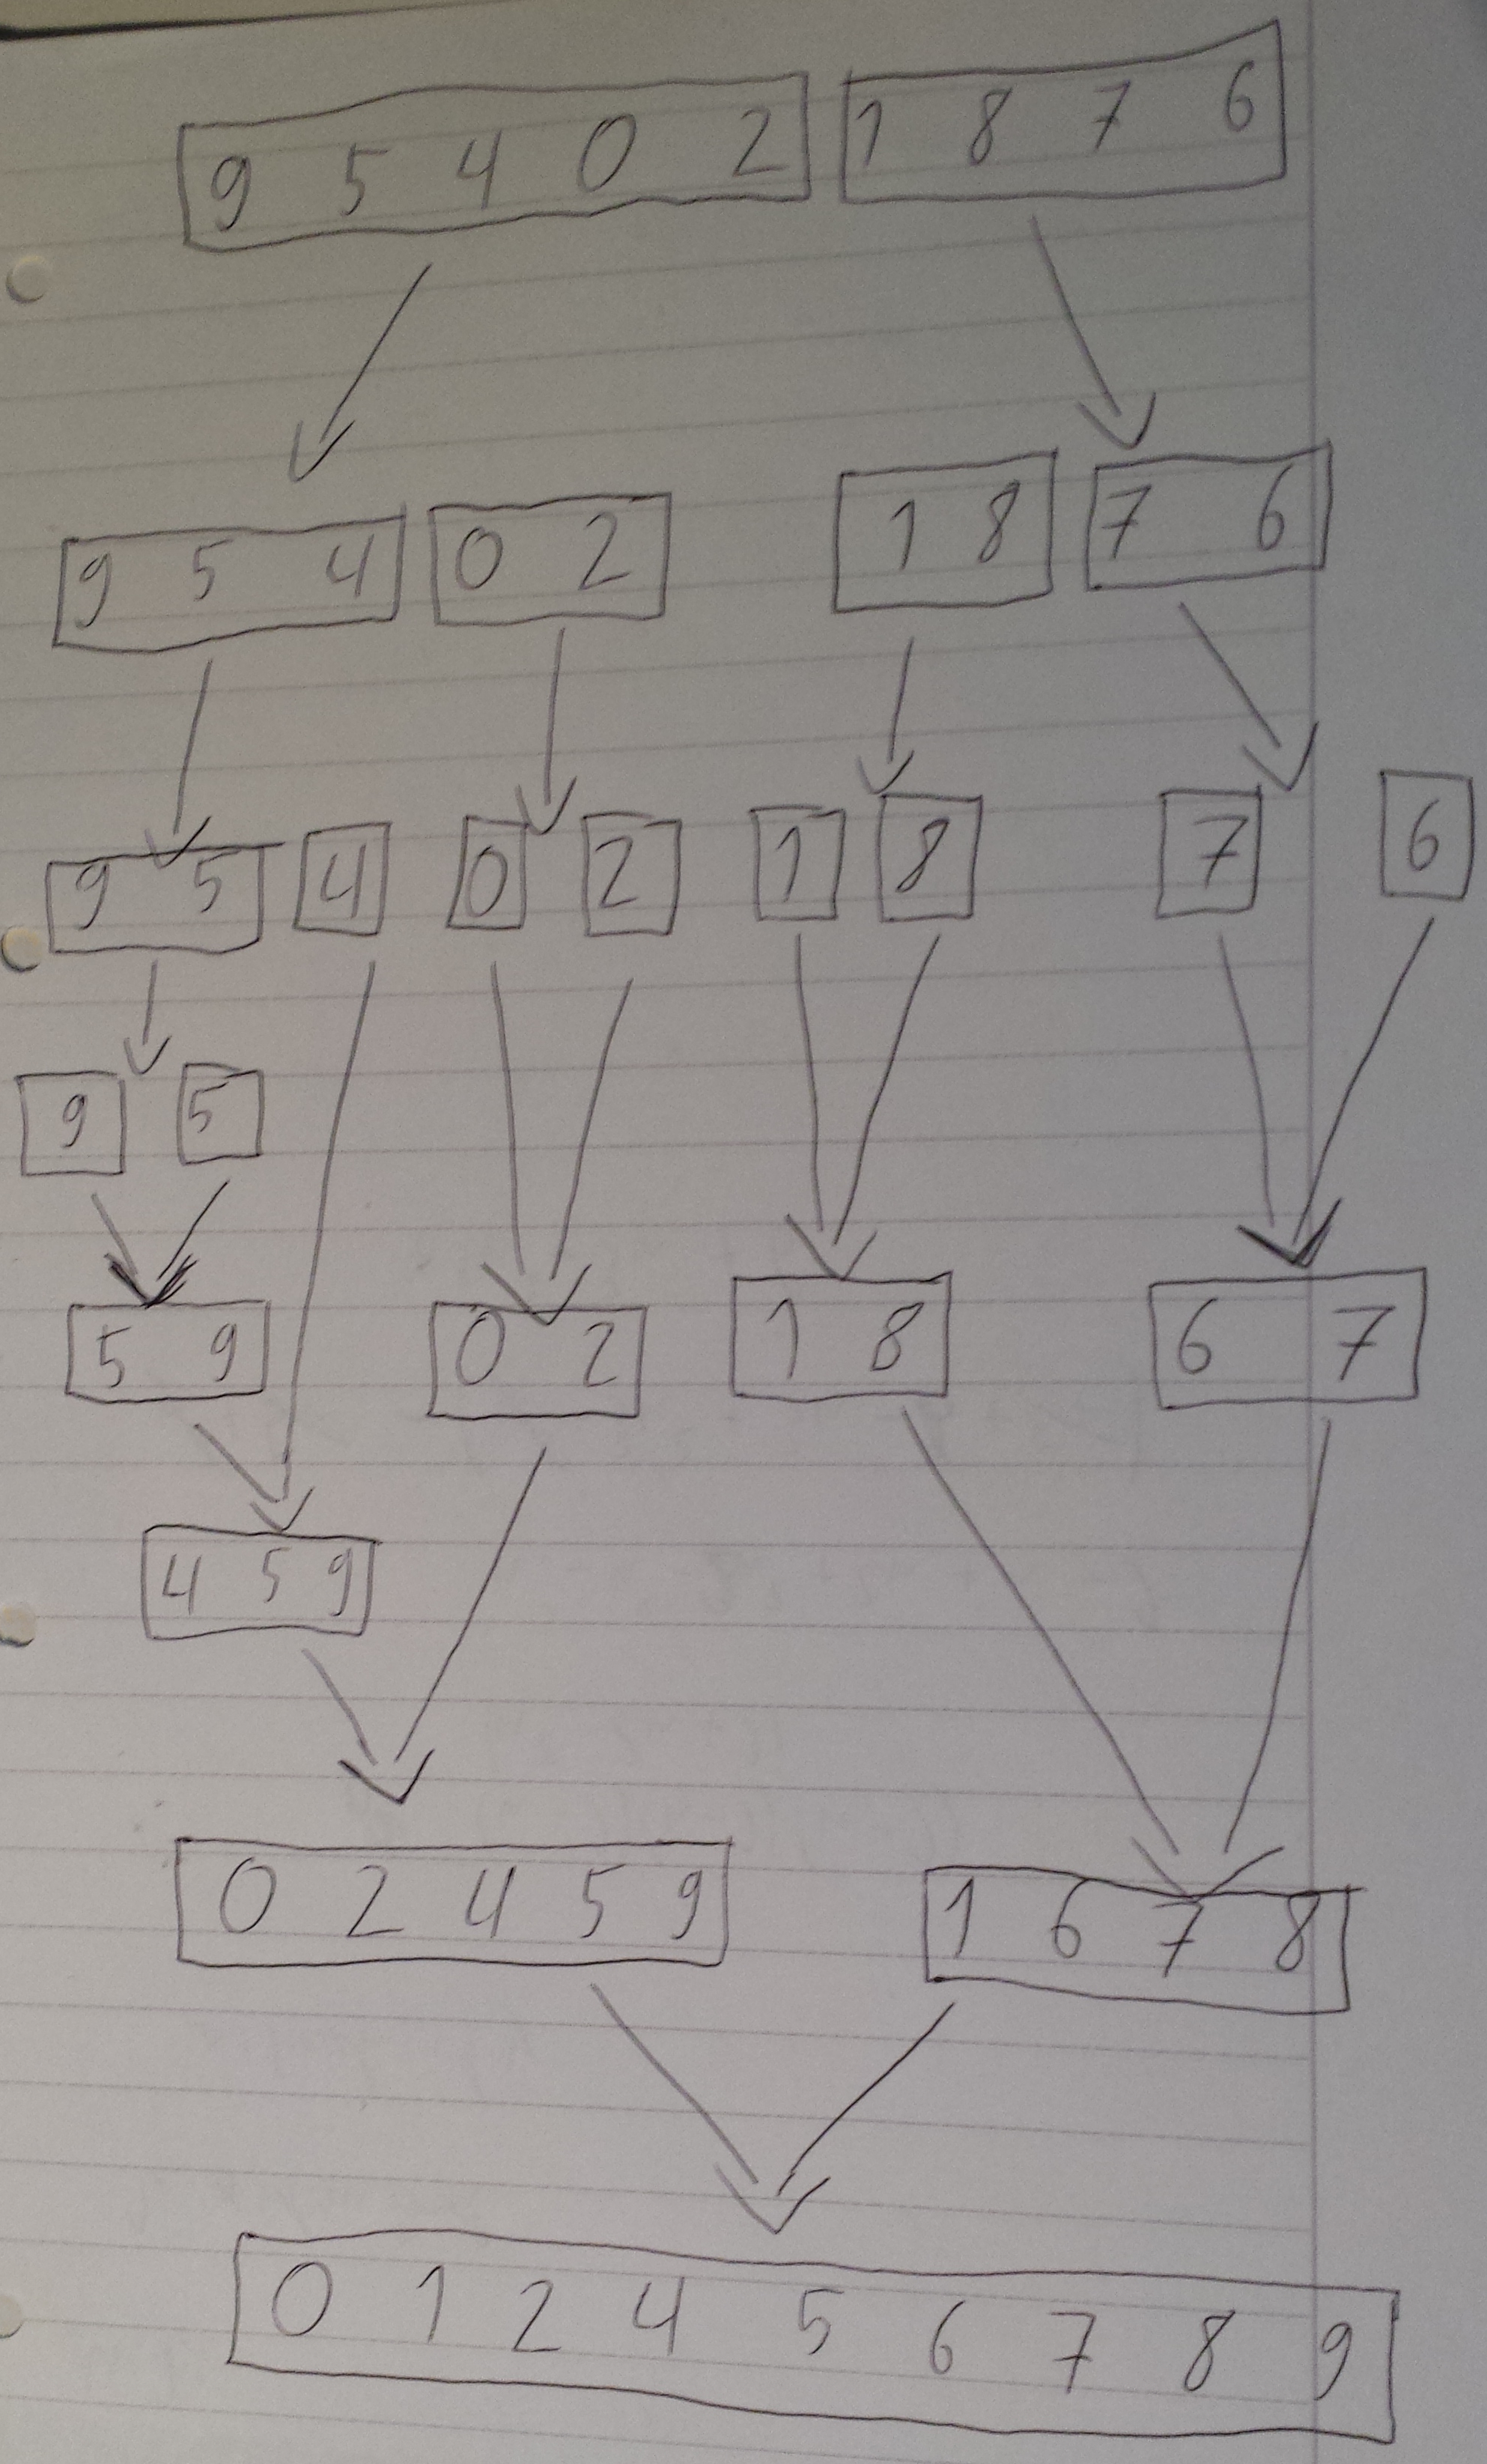
\includegraphics[width=400pt]{3_4}
\end{figure}

\end{document}